% begin module sequence-squeeze-theorem
\begin{frame}
The Squeeze Theorem also works for sequences:
\begin{theorem}[The Squeeze Theorem for Sequences]
If $a_n\leq b_n\leq c_n$ for $n \geq n_0$ and $\lim_{n\to\infty} a_n = L = \lim_{n\to\infty}c_n$, then $\lim_{n\to\infty}b_n=L$.
\end{theorem}
\begin{center}
\psset{xunit=1cm, yunit=1cm}
\begin{pspicture}(-0.5,-0.5)(10, 3)
\tiny
\fcAxesStandard{-0.5}{-0.5}{7}{3}
\rput[b](0,3.1){$a$}
\rput[l](7.1,0){$n$}
\multido{\na=1+1}{35}{%
\pstVerb{2 dict begin /na \na\space def /t na 0.2 mul def}%
\fcFullDot[scale=0.6, linecolor=red]{t }{1 t 1 add div 1 add}
\fcFullDot[scale=0.6, linecolor=black]{t }{1 t 1 add div t 180 mul sin mul 1 add}
\fcFullDot[scale=0.6, linecolor=blue]{t }{-1 t 1 add div 1 add}
\pstVerb{end}%
}%
\psline[linewidth =0.4pt, linestyle=dotted, linecolor=blue](0, 1)(7, 1)
\rput[r](-0.1, 1){$L$}
\rput[b](0.2, 2){\color{red}$c_n$}
\rput[t](0.2, 1.4){\color{black}$b_n$}
\rput[b](0.2, 0.4){\color{blue}$c_n$}
\end{pspicture}
%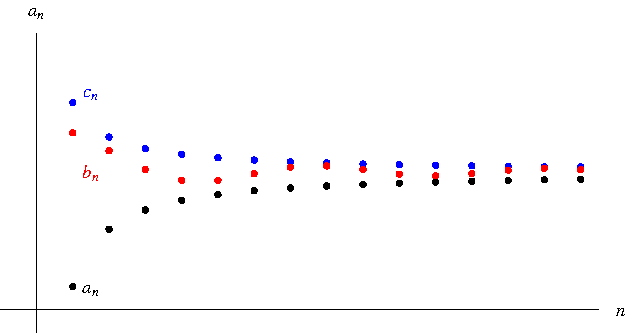
\includegraphics[width=8cm]{sequences/pictures/12-01-squeeze.pdf}%
\end{center}
\uncover<2->{%
%Here is a corollary to the Squeeze Theorem for sequences:
\begin{corollary}
If $\lim_{n\to\infty} |a_n| = 0$, then $\lim_{n\to\infty}a_n = 0$.
\end{corollary}
}%
\end{frame}
% end module sequence-squeeze-theorem
